\documentclass[a4paper,oneside]{book} 
% the 'oneside' option makes viewing on a computer easier, as both inner and outer margins are equal. Change this while printing.

\usepackage{amsmath,amssymb}
\usepackage{hyperref}
\usepackage{amscd}
\usepackage{amsthm}
\usepackage{color}

\usepackage[T1]{fontenc}

\usepackage{enumerate} % Customize the enumerate environment
\usepackage{mathtools} % for \prescript

%\usepackage{cite}
\usepackage{bm} 

\usepackage[vcentermath]{youngtab} % Excellent package for young diagrams

% For compact lists. Provides the environments 
%   itemize*, enumerate*, description*
% with lesser spacing between items.
\usepackage{mdwlist} 
\usepackage{enumerate} 

\usepackage{mathtools} % For 'Aboxed' command

% Theorem-like environments
\usepackage{amsthm}
\theoremstyle{definition}
\newtheorem{definition}{Definition}

\theoremstyle{plain}
\newtheorem{theorem}{Theorem}
\newtheorem{corollary}{Corollary}
\newtheorem{conjecture}{Conjecture}
\newtheorem{lemma}{Lemma}
\newtheorem{proposition}{Proposition}

% TikZ
\usepackage{tikz}
\usepackage{tikz-cd} % Commutative Diagrams in TikZ
\usetikzlibrary{positioning}
\usetikzlibrary{decorations.pathreplacing} % for curly braces
\usetikzlibrary{decorations.pathmorphing} % for squiggly arrows
\usetikzlibrary{calc} % for coordinate calculation
% Tikz Style for Commutative Diagrams
\tikzset{
    commutative diagram/.style={
            node distance=2cm,auto,
            arrow/.style={-stealth},
            exists/.style={-stealth,densely dotted}
        }
    }

% This compactifies a list by removing unnecessary whitespace
\newcommand\makethislistcompact{
        \setlength{\itemsep}{0pt}%
        \setlength{\parskip}{0pt}%
        %\setlength{\topsep}{50pt} 
        %\setlength{\partopsep}{10pt}
        %\setlength{\parsep}{50pt}
}
% Framed environments
\usepackage[framemethod=tikz]{mdframed}

% Common operators
\DeclareMathOperator\GL{GL}  % General Linear Group
\DeclareMathOperator{\Image}{Im} % Image
\DeclareMathOperator{\Coker}{Coker} % Cokernel 
\DeclareMathOperator{\Ker}{Ker} % Kernel
\DeclareMathOperator{\Tr}{Tr} % Trace
\DeclareMathOperator{\Hom}{Hom} % Homomorphisms
\DeclareMathOperator{\End}{End} % Endomorphisms
\DeclareMathOperator{\Aut}{Aut} % Automorphisms
% Commonly used sets
\newcommand{\CC}{\mathbb{C}}
\newcommand{\RR}{\mathbb{R}}
\newcommand{\ZZ}{\mathbb{Z}}
\newcommand{\HH}{\mathbb{H}}
\newcommand{\FF}{\mathbb{F}}
\newcommand{\uhp}{\mathcal{H}}
\newcommand{\SL}{\text{SL}}

\renewcommand{\>}{\rangle}
\newcommand{\<}{\langle}

% Some semantically named symbols
\newcommand\isomorphic\cong

% Meta-notes
\newcommand\Solution[2]{\emph{[Solution to Exercise #1 in #2]}}
\newcommand\Todo[1]{\begin{color}{red}{#1}\end{color}}
\newcommand{\tocheck}[1]{{\color{red} #1}}
\newcommand{\comment}[1]{{\color{cyan} #1}}

% Environment for "physical insights"
\newenvironment{insight}
  {\begin{mdframed}[%style=2,%
      leftline=true,
      rightline=true,
      topline=false,
      bottomline=false,
      leftmargin=2em,
      rightmargin=2em,%
      innerleftmargin=1em,
      innerrightmargin=1em,
      linewidth=2pt,%
      linecolor=white!70!black,%
      %backgroundcolor=white!99!black, %
      skipabove=7pt,skipbelow=7pt]\small}
  {\end{mdframed}}

%%%%%%%%%%%%%%%%%%%%%%%%%%%%%%%%


\setcounter{secnumdepth}{1}
\title{Differential Geometry}
\author{Hersh Singh}

\begin{document}
\maketitle
\chapter{Basics}
\label{cha:basics}
\begin{definition}
    A topological space $M$ is called Haursdoff if any two points in it can be seperated by open sets. Explicitly, for any two points $p,q\in M $, there must be open neighbourhoods of $U,\, U'$ of $p,q$ respectively such that $U\cap U'=\varnothing$.
\end{definition}

\section{Manifold}
\label{sec:manifold_}

$M$ is an $n$ dimensional topological manifold if it 
\begin{enumerate}[(i)]
    \makethislistcompact
    \item is \emph{Haursdoff},
    \item has a countable basis for topology, that is, it is \emph{second countable},
    \item is locally homeomorphic to $\RR^n$.\\
\end{enumerate}

A basis for a topological space $M$ is just an a family of open sets $\{U_\alpha|\alpha\in I\}$ such that $M=\bigcup_{\alpha\in I}U_\alpha$.

\begin{insight}
   The dimension of an $n$-dimensional manifold is unique. 
\end{insight}

\subsection{Coordinate Charts}
\label{sub:coordinate_charts}
One of main motivations of a manifold is to find a space which looks locally euclidean. This section makes that explicit.

A pair $(U,\varphi)$ where $U\in M$ is open and $\varphi: U \to \RR^n$ is a homeomorphism is called a \emph{coordinate chart}. By definition of a manifold, any point $p\in M$ is contained in at least one such open set $U\in M$.

Given a pair $(U,\varphi)$, we call $U$ the \emph{coordinate domain} or \emph{coordinate neighbourhood} of each of its points. The set $U$ is called a \emph{coordinate ball} or a \emph{coordinate cube} if the image $\varphi(U)$ is an open ball or an open cube in $\RR^n$, respectively.

\subsection{Topological Properties of Manifolds}
\label{sub:topological_properties_of_manifolds}

\subsection{Smooth Structures}
\label{sub:smooth_structures}
We can intuitively guess what a smooth map on the euclidean space means.
A map $F: V\to U$, where $U\in \RR^n,\ V\in \RR^m$ are open subsets, is said to be \emph{smooth} if all its partial derivatives are continuous in all orders. If in addition $F$ is bijective and has a smooth inverse map, then it's called a \emph{diffeomorphism}.

Now, here's how we extend concept of smoothness to manifolds.

We have $M$, a topological $n$-manifold. 
\begin{center}
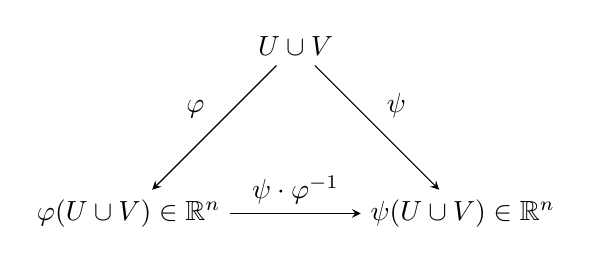
\begin{tikzpicture}[commutative diagram, node distance=3cm]
    \node (uv) {$U\cup V$};
    \node (image1) [below left of=uv]{$\varphi(U\cup V)\in \RR^n$};
    \node (image2) [below right of=uv]{$\psi(U\cup V)\in \RR^n$};
    \draw [arrow] (uv) -- (image1) node [midway,auto=right] {$\varphi$};
    \draw [arrow] (uv) -- (image2) node [midway] {$\psi$};
    \draw [arrow] (image1) -- (image2) node [midway] {$\psi\cdot\varphi^{-1}$};
\end{tikzpicture}
\end{center}
We already know how to talk about the smoothness of the map $\psi\cdot\varphi^{-1}$, since its just a map on the euclidean space. Lets call this the \emph{transition map} from $\varphi$ to $\psi$. Two charts $(U,\varphi)$ and $(V,\psi)$ are said to be smoothly compatible if either $U \cup V =\varnothing$ or the if transition map $\psi\cdot\varphi^{-1}$ is a diffeomorphism.

We define an \emph{atlas for $M$} as a collection of charts whose domains cover $M$. An atlas $\mathcal A$ is called a \emph{smooth atlas} if any two charts in $\mathcal A$ are smoothly compatible with each other.

\begin{insight}
   more here 
\end{insight}












%This makes explicit the idea of being \emph{locally homeomorphic} to $\RR^n$. 





\section{Tangent Space}
\label{sec:tangent_space}


    

\appendix
\chapter{References}
\begin{enumerate*}
    \item Introduction to Differential Topology by Brocker and Janich
\end{enumerate*}

    
\end{document}



